% Teilauswertung X

\section{Aufnahme der Sensitized Emission}

In diesem Teil der Auswertung sollen die Bilder der Sensitized Emission und der FRET-Effizienz bestimmt werden.

\subsection{Bestimmung der Korrekturfaktoren}

Zu aller erst ist es notwendig Korrekturfaktoren zu bestimmen, um sogenannte Crosstalk Verunreinigungen zu beheben. Eine genauere Erklärung was Crosstalk Verunreinigungen sind und warum sie existieren findet sich in Abschnitt \ref{sec:verunreinigung}. \\

Folgende Korrekturfaktoren werden benötigt: 
\begin{align}
    \label{eq:korfakA}
    \alpha = \frac{D_{YFP}}{A_{YFP}}\\
    \beta = \frac{S_{CFP}}{D_{CFP}}\\
    \gamma = \frac{S_{YFP}}{A_{YFP}}\\
    \delta = \frac{D_{YFP}}{s_{YFP}}
    \label{eq:korfakB}
\end{align}

Bedeutung der Formelsymbole: 
\begin{itemize}
    \item D: Mit Anregung und Detektion des Donors
    \item A: Mit Anregung und Detektion des Akzeptors
    \item S: Mit Anregung des Donors und Detektion des Akzeptors
\end{itemize}

Erklärung der Indizes:
\begin{itemize}
    \item CY: Probe enthält beide Farbstoffe
    \item YFP: Probe enthält nur YFP
    \item CFP: Probe enthält nur CFP
\end{itemize}

\newpage
Im Folgenden soll nun anhand eines Beispiels die Vorgehensweise demonstriert werden, mit der die jeweiligen Werte für die Korrekturfaktoren bestimmt werden.\\

Als Beispiels haben wir den Wert $D_{YFP}$ ausgewählt.\\
Zuerst wird ein Bild einer Probe aufgenommen, welches die passenden Farbstoffe enthält (hier nur YFP). Außerdem wird der passende Aufnahmemodus gewählt, hier Anregung und Detektion des Donors.\\
Danach werden in diesen mithilfe der Programms Fiji die Mittelwerte bestimmter ROI's (Region of interest) bestimmt. Eine ROI wird in einem zellfreien Bereich platziert, um den Wert des Hintergrundes zu erfassen können ($D_{YFP(bg)}$). Die andere ROI wird um die Membran der Zelle gelegt ($D_{YFP(mb)}$). Dies wird in Abbildung \ref{fig:VerschROI} an einem Beispiel verdeutlicht.

\begin{figure}[h]
    \centering
    \begin{subfigure}[]{0.45\textwidth}
        \centering
        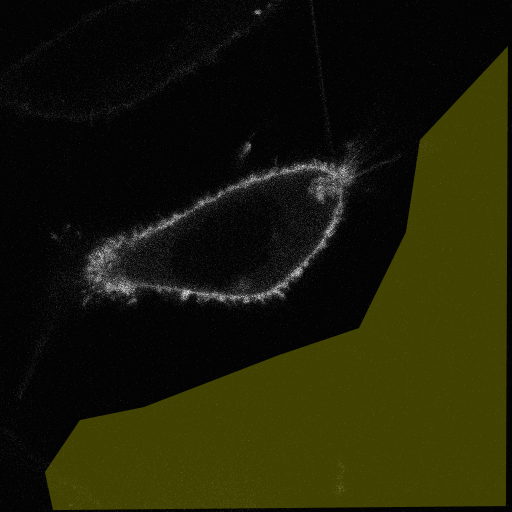
\includegraphics[width=\textwidth]{Paul/D-CY-bg.png}
        \caption{Beispiel: ROI des Hintergrundes}
    \end{subfigure}
    \hfill 
    \begin{subfigure}[]{0.45\textwidth}
        \centering
        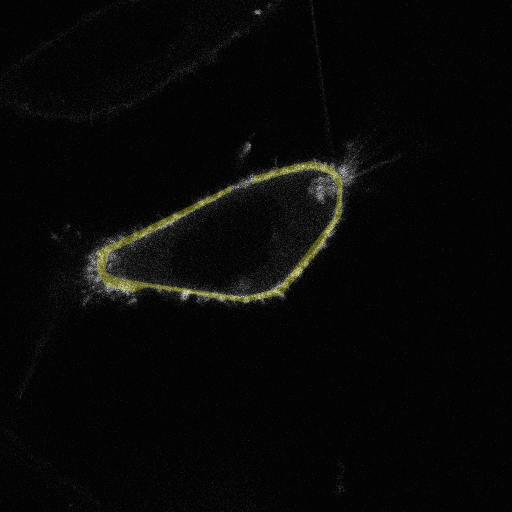
\includegraphics[width=\textwidth]{Paul/D-CY-zm.png}
        \caption{Beispiel: ROI der Zellmembran}
    \end{subfigure}
    \caption{Verschiedene ROI in $D_{CY}$ (hier: Zelle CY1)}
    \label{fig:VerschROI}
\end{figure}

Um nun der Wert zu bestimmen wird der Hintergrundwert abgezogen: 
\begin{align}
    D_{YFP} = D_{YFP(mb)} - D_{YFP(bg)}
\end{align}

\newpage
Dieser Vorgang wurde in analoger Weise für alle anderen Werte wiederholt. Dannach werden die Gleichungen \ref{eq:korfakA} bis \ref{eq:korfakB} verwendet um die Korrekturfaktoren zu berechnen. Dabei haben sich folgende Werte ergeben: \\

\begin{table}[h]
    \centering
    \begin{tabular}{c|c|c|c}
         Messung Nr. &        $D_{CFP}$ &           $S_{CFP}$ &      $\beta$ \\ \hline\hline
               1 &  102.466 &      18,805 &  0.183524 \\\hline
               2 &   68.186 &      12,936 &  0.189716 \\\hline
               3 &   15.184 &       2,796 &  0.184141 \\\hline
               4 &   38.030 &       6,681 &  0.175677 \\\hline
               5 &   27.955 &        4,86 &  0.173851 \\\hline
               6 &   18.747 &       3,229 &  0.172241 \\\hline
               7 &   89.738 &      16,416 &  0.182933 \\\hline
               8 &   56.398 &      10,034 &  0.177914 \\\hline
               9 &   58.660 &      10,779 &  0.183754 \\\hline
              10 &   50.819 &       8,977 &  0.176647 \\\hline
        \end{tabular}
    \caption{Messungen für CFP markierte Zellen zur Bestimmung von $\beta$}
\end{table}

\begin{table}[h]
    \centering
    \begin{tabular}{c|c|c|c|c|c|c}
         Messung Nr. &  $D_{YFP}$ & $A_{YFP}$ & $S_{YFP}$ &     $\alpha$ &     $\gamma$ &     $\delta$ \\\hline\hline
         1 &  1.685 &  179.276 &  97.906 &  0.009399 &  0.546119 &  0.017210 \\\hline
         2 &  0.371 &   40.330 &  17.076 &  0.009199 &  0.423407 &  0.021726 \\\hline
         3 &  0.529 &   94.979 &  38.451 &  0.005570 &  0.404837 &  0.013758 \\\hline
         4 &  0.538 &   60.703 &  25.409 &  0.008863 &  0.418579 &  0.021174 \\\hline
         5 &  0.429 &   75.727 &  32.435 &  0.005665 &  0.428315 &  0.013226 \\\hline
         6 &  0.533 &   63.920 &  27.325 &  0.008339 &  0.427487 &  0.019506 \\\hline
         7 &  0.651 &  114.199 &  48.084 &  0.005701 &  0.421054 &  0.013539 \\\hline
         8 &  0.490 &   31.834 &  13.232 &  0.015392 &  0.415656 &  0.037031 \\\hline
         9 &  0.598 &   80.300 &  34.689 &  0.007447 &  0.431993 &  0.017239 \\\hline
        10 &  0.607 &   72.924 &  30.036 &  0.008324 &  0.411881 &  0.020209 \\\hline
        \end{tabular}
    \caption{Messungen für YFP markierte Zellen zur Bestimmung von $\alpha$, $\gamma$ und $\delta$}
\end{table}

Somit ergeben sich folgende Mittelwerte für die Korrekturfaktoren: 
\begin{align}
    \alpha = (0,008 \pm 0,003)\\
    \beta = (0,180 \pm 0,006)\\
    \gamma = (0,43 \pm 0,04)\\
    \delta = (0,019 \pm 0,007)
\end{align}
Der Fehler wurde über die Standardabweichung berechnet.

\newpage
\subsection{Bestimmung der Sensitized Emission und FRET-Effizienz Bilder}

Mithilfe der Korrekturfaktoren können die Werte und Bilder der Sensitized Emission und der FRET-Effizienz, unter Verwendung folgender Formeln und des Programms Fiji, errechnet werden.
\begin{align}
    SE &= \frac{S_{CY} - \beta \cdot D_{CY} - (\gamma -\alpha \beta)\cdot A_{CY}}{1 - \beta \delta} \\
    E &= \frac{SE}{\sqrt{A_{CY} \cdot D_{CY}}}
\end{align}


Folgende Werte haben sich aus der Verwendung der Formel ergeben:\\

\begin{table}[h]
    \centering
    \begin{tabular}{c|c|c|c|c|c}
         Zelle Nr. &       D &            S &        A &         SE &         E \\\hline\hline
               1.0 &  78.989 &       54,464 &   78.642 &  43.176840 &  0.547823 \\\hline
               2.0 &  48.876 &       29,519 &   44.437 &  22.002979 &  0.472130 \\\hline
               3.0 &  40.770 &       28,091 &   40.630 &  22.037036 &  0.541451 \\\hline
               4.0 &  35.516 &       24,841 &   40.206 &  19.538192 &  0.517043 \\\hline
               5.0 &  31.778 &       22,537 &   36.237 &  17.769305 &  0.523638 \\\hline
               6.0 &  65.660 &       29,534 &   36.419 &  18.742015 &  0.383267 \\\hline
               7.0 &  42.112 &       32,539 &   53.054 &  26.599006 &  0.562734 \\\hline
               8.0 &  47.894 &       27,762 &   40.689 &  20.289197 &  0.459606 \\\hline
               9.0 &  34.241 &       30,621 &   50.415 &  26.055755 &  0.627120 \\\hline
              10.0 &  17.931 &        59,38 &  127.373 &  60.430551 &  1.264491 \\\hline
              11.0 &  36.992 &         27,7 &   41.517 &  22.350672 &  0.570327 \\\hline
              12.0 &  29.925 &       28,352 &   47.459 &  24.437686 &  0.648461 \\\hline
              14.0 &   5.800 &        8,738 &   16.353 &   7.876263 &  0.808737 \\\hline
              15.0 &  31.486 &       28,789 &   45.679 &  24.606828 &  0.648841 \\\hline
              16.0 &  22.483 &       19,491 &   33.136 &  16.280748 &  0.596482 \\\hline
              17.0 &  23.921 &       18,978 &   29.997 &  15.443600 &  0.576527 \\\hline
              18.0 &  22.910 &       16,174 &   25.549 &  12.599973 &  0.520799 \\\hline
        \end{tabular}
        \caption{Ermittelte D, S, A, SE und E Werte der CY markierten Zellen.}
        \label{tab:CYSEE}
\end{table}

Für Mittelwert und Standardabweichung gilt: 
\begin{align*}
    SE = (23 \pm 12) \qquad E = (0,6 \pm 0,2)
\end{align*}
In der Tabelle \ref{tab:CYSEE} bei Zelle Nr. 10 ist jedoch ein Wert für die FRET Effizienz von deutlich über eins zu sehen. Dies macht für diesen Wert jedoch keinen Sinn und ist somit wahrscheinlich ein Messfehler.

\newpage
Nachfolgend sind ausgewählte Bilder abgebildet die aus diesen Formeln resultieren.

\begin{figure}[h]
    \centering
    \begin{subfigure}[]{0.45\textwidth}
        \centering
        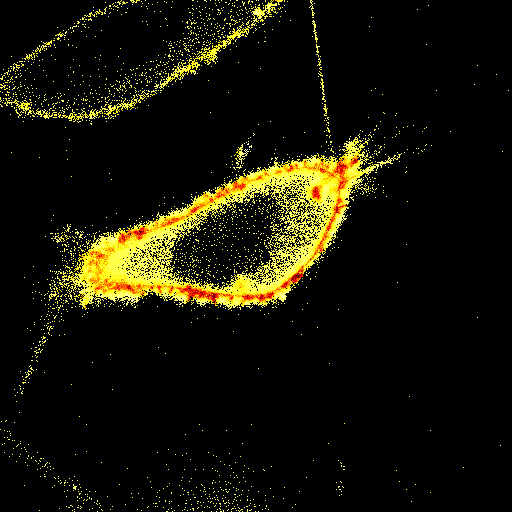
\includegraphics[width=\textwidth]{Paul/SE1.png}
        \caption{SE Bild der Aufnahme CY1}
    \end{subfigure}
    \hfill 
    \begin{subfigure}[]{0.45\textwidth}
        \centering
        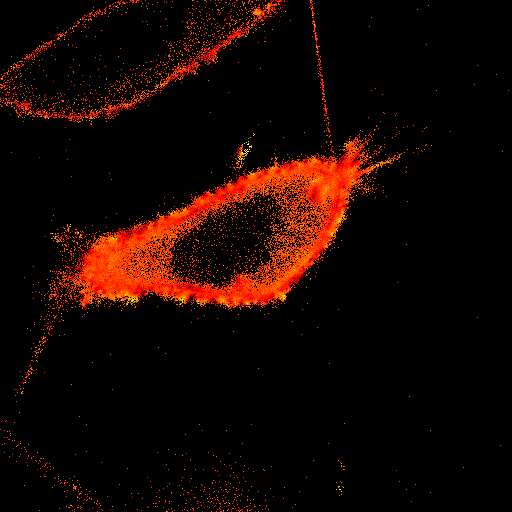
\includegraphics[width=\textwidth]{Paul/E1.png}
        \caption{E Bild der Aufnahme CY1}
    \end{subfigure}
    \caption{Zelle CY1 in SE und E}
    \label{fig:CY1}
\end{figure}

Für die Zelle in Abbildung \ref{fig:CY1} würde wieder eine ROI um die Zellmembran gelegt. Der mittlere Wert der ROI's hat folgendes ergeben: 

\begin{align*}
    \overline{SE} = 9,129 \qquad \overline{E} = 0,195
\end{align*}

Vergleicht man diese Werte mit den rechnerischen ermittelten aus Tabelle \ref{tab:CYSEE}, so fallen deutliche Unterschiede auf.

\newpage
\begin{figure}[h]
    \centering
    \begin{subfigure}[]{0.45\textwidth}
        \centering
        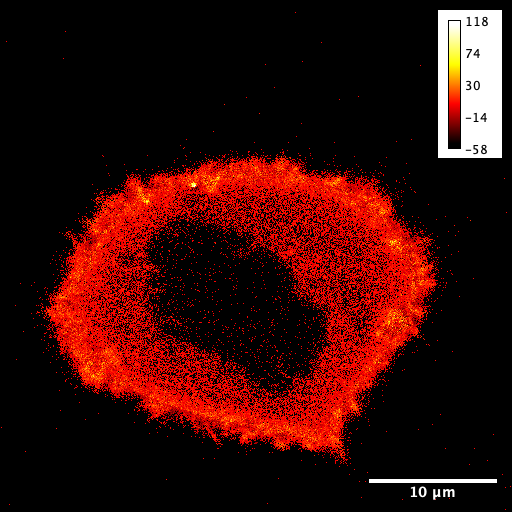
\includegraphics[width=\textwidth]{Paul/SE3.png}
        \caption{SE Bild der Aufnahme CY3}
    \end{subfigure}
    \hfill 
    \begin{subfigure}[]{0.45\textwidth}
        \centering
        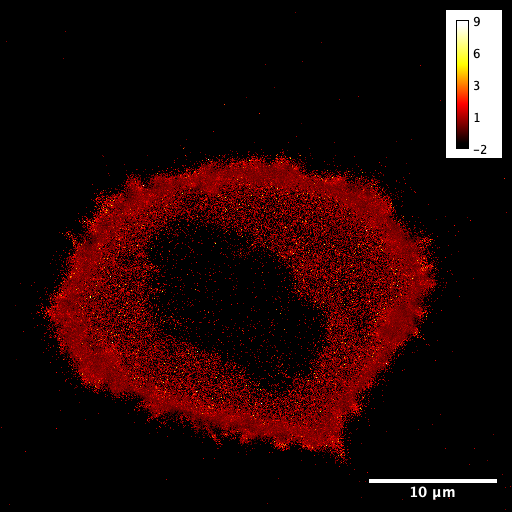
\includegraphics[width=\textwidth]{Paul/E3.png}
        \caption{E Bild der Aufnahme CY3}
    \end{subfigure}
    \caption{Zelle CY3 in SE und E}
    \label{fig:CY3}
\end{figure}

Für die Zelle in Abbildung \ref{fig:CY3} wurden die Mittelwerte analog ermittelt: 
\begin{align*}
    \overline{SE} = 3,951 \qquad \overline{E} = 0,200
\end{align*}
Auch hier fallen deutliche Unterschiede ins Auge.

\subsection{Abstand der Fluorophore}
Im Theorieteil wurde mit Gleichung \ref{eq:effizienz} eine andere Gleichung für die FRET Effizienz angegeben. 
\begin{align}
    E = \frac{R_F^6}{R_F^6+R^6}
\end{align}
Durch Umstellen dieser Formel kann folgende Gleichung für den mittleren Abstand angegeben werden: 
\begin{align}
    R = \sqrt[6]{\frac{R_F^6}{E} - R_F^6} 
\end{align}
Wobei $R_F$ der Försterradius ist. Dieser müsste noch bestimmt werden, um den mittleren Abstand zu berechnen.

\newpage
\section{Donoremission nach Akzeptorbleichung}
In diesem Versuchsteil soll die FRET-Effizienz ermittelt werden, indem man die Donorfluoreszenz vor und nach dem Bleichen der jeweiligen Probe misst. Die Formel zur Berechnung der FRET-Effizienz ist folgende: 
\begin{align}
    E = 1 - \frac{D_{CY,pre}}{D_{CY,post}}
    \label{eq:FREE}
\end{align}

Die eigentliche Versuchsdurführung wurde größtenteils durch einen speziellen Assistenten des Kontrollprogramms ausgeführt. Im Voraus musste nur eine passende Zelle ausgewählt werden und die verschiedenen ROI's (wie in Abbildung \ref{fig:ROIs} gezeigt) eingezeichnet werden.
\begin{itemize}
    \item ROI 1: Der zu bleichende Bereich
    \item ROI 2: Die Zellmembran (oder ein Teil)
    \item ROI 3: Eine helle Stelle
\end{itemize}

\begin{figure}[h]
    \centering
    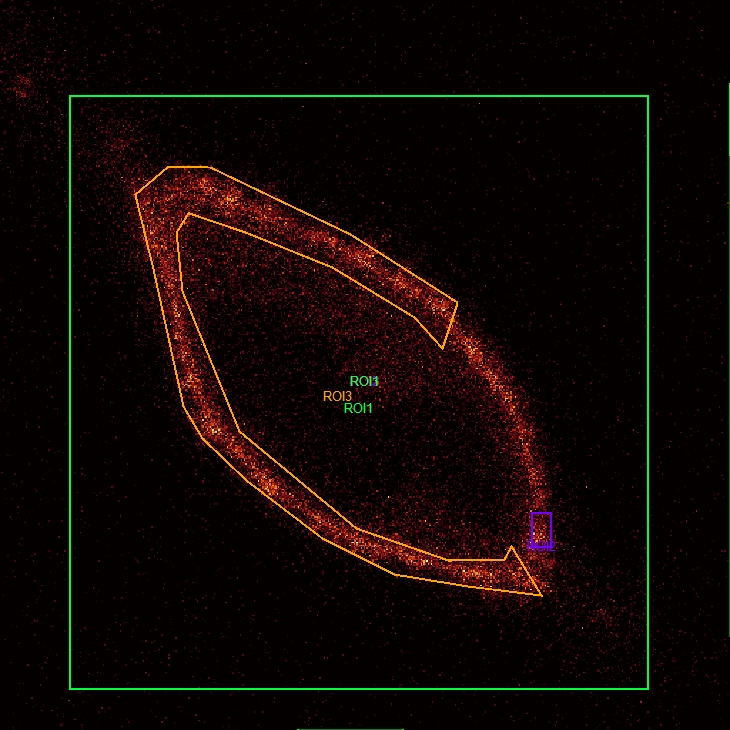
\includegraphics[width=0.5\textwidth]{Paul/BleachCY-ROI.jpg}
    \caption{Darstellung der verschiedenen ROI's}
    \label{fig:ROIs}
\end{figure}

Mithilfe eines Pythonskripts wurde die Formel \ref{eq:FREE} auf die einzelnen ROI's der Verschiedene Dateien, die mittels des Messprogramms erstellt wurden, angewendet. Dabei ergaben sich folgende Werte: 
\begin{table}[h]
    \centering
    \begin{tabular}{c|c|c|c}
          Datenreihe &     ROI 1 &     ROI 2 &     ROI 3 \\\hline\hline
          CY-1-D.csv &  0.003505 &  0.030953 & -0.000090 \\\hline
          CY-10-D.csv &  0.026029 &  0.135385 &  0.072495 \\\hline
           CY-2-D.csv &  0.053433 &  0.059482 &  0.048435 \\\hline
           CY-3-D.csv &  0.012226 &  0.032995 &  0.110722 \\\hline
           CY-4-D.csv &  0.024620 &  0.036954 & -0.000083 \\\hline
           CY-5-D.csv & -0.018922 &  0.053814 &  0.053266 \\\hline
           CY-6-D.csv &  0.021359 &  0.048867 &  0.069277 \\\hline
           CY-7-D.csv &  0.035247 &  0.084725 &  0.069380 \\\hline
           CY-8-D.csv &  0.027918 &  0.141295 &  0.051616 \\\hline
           CY-9-D.csv &  0.064711 &  0.024094 &  0.129895 \\\hline
        \end{tabular}
        \caption{E-Werte für die verschiedenen ROIs der CY markierten Zellen}
\end{table}

\begin{table}[h]
    \begin{tabular}{c|c|c|c}
        Datenreihe &     ROI 1 &     ROI 2 &     ROI 3 \\\hline\hline
         YFP-1.csv & -0.749496 & -1.370115 & -1.415964 \\\hline
         YFP-2.csv & -2.436369 & -6.608389 & -3.299554 \\\hline
         YFP-3.csv & -1.907869 & -3.509338 & -2.912716 \\\hline
        \end{tabular}
\end{table}
